\documentclass[11pt]{article}
% Shared preamble for the three living documents.
\usepackage[T1]{fontenc}
\usepackage{lmodern}
\usepackage[utf8]{inputenc}
\usepackage[margin=2.4cm]{geometry}
\usepackage{microtype}
\usepackage{amsmath,amssymb}
\usepackage{siunitx}
\usepackage{booktabs}
\usepackage{enumitem}
\usepackage{xcolor}
\usepackage{tikz}
\usetikzlibrary{arrows.meta,positioning,calc}
\usepackage{listings}
\usepackage[backend=biber,style=numeric,sorting=none]{biblatex}
\addbibresource{references.bib}
\usepackage[colorlinks=true,linkcolor=blue!50!black,citecolor=green!40!black,urlcolor=blue!60!black]{hyperref}

\newcommand{\vect}[1]{\mathbf{#1}}
\newcommand{\unitv}[1]{\hat{\mathbf{#1}}}
\newcommand{\dd}{\mathrm{d}}
\newcommand{\project}{Physics Sandbox}

\lstset{basicstyle=\ttfamily\small,columns=flexible,keepspaces=true,breaklines=true,frame=single,framerule=0.3pt}
\setlist{itemsep=2pt}
\setlength{\emergencystretch}{3em}

\title{\project{} --- Code Notes}
\author{Living document}
\date{Last updated: \today}

\begin{document}
\maketitle
\noindent This document describes how the software is organised, why it is organised
that way, and how to build, test and extend it. Each implementation step adds a section.

\tableofcontents

\section{Goals that shape the design}
\begin{itemize}
  \item \textbf{Runs almost everywhere.} Web first, then desktop (Windows/Linux/macOS) and Android
        wrappers around the same web app. Must stay usable on low-end phones.
  \item \textbf{Portable physics core.} The core has no browser or rendering dependencies so it can
        be ported to Rust/WebAssembly~\cite{wasmbindgen} later without touching the UI.
  \item \textbf{Deterministic and testable.} Simulation is a pure function of its inputs.
\end{itemize}

\section{Technology stack}
\begin{center}
\begin{tabular}{@{}lll@{}}
\toprule
Concern & Choice & Why \\ \midrule
Language & TypeScript (strict)~\cite{tshandbook} & types, runs in every browser \\
Build / dev server & Vite~\cite{vite} & fast, zero-config, static output \\
3D rendering & three.js, WebGL\,2~\cite{threejs} & widest GPU support; WebGPU later \\
Camera & OrbitControls~\cite{orbitcontrols} + own rig & orbit/pan/zoom, mouse and touch \\
Plots & uPlot~\cite{uplot} & $\approx$\SI{50}{kB}, handles $10^5$ points smoothly \\
Tests & Vitest~\cite{vitest} & same toolchain as Vite \\
UI & plain DOM + CSS & no framework weight on low-end devices \\
Docs & \LaTeX{} + biber & these documents \\ \bottomrule
\end{tabular}
\end{center}

\section{Milestone 1: a ball on a table}

\subsection{Directory layout}
\begin{lstlisting}
src/
  core/      pure physics: vec3, types, forces, contact, dynamics,
             world, history, kinematics, defaults   (no DOM, no three.js)
  sim/       controller.ts (timeline, commands, events), emitter.ts
  render/    three.js: viewport, scene, table, ball, forceArrow,
             camera (CameraRig), renderer, quality
  ui/        DOM panels: forcePanel, plotPanel, settingsPanel,
             timeline, viewControls, hud, dom helpers, styles.css
  theme.ts   colours shared by 3D view and plots
  main.ts    wiring + frame loop
tests/core/  Vitest unit tests
docs/        physics.tex, math.tex, code.tex, references.bib
\end{lstlisting}

\subsection{Layers}
\begin{center}
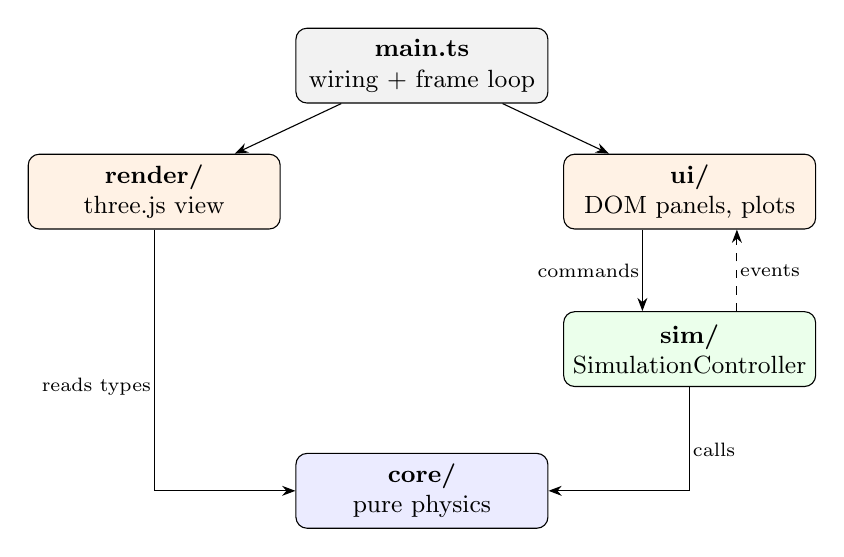
\begin{tikzpicture}[
  box/.style={draw, rounded corners, minimum width=3.2cm, minimum height=0.95cm, align=center, font=\small},
  lbl/.style={font=\scriptsize, fill=white, inner sep=1pt},
  >=Stealth]
  \node[box, fill=gray!10]   (main)   at (0, 4.2)  {\textbf{main.ts}\\wiring + frame loop};
  \node[box, fill=orange!10] (render) at (-3.4, 2.6) {\textbf{render/}\\three.js view};
  \node[box, fill=orange!10] (ui)     at (3.4, 2.6)  {\textbf{ui/}\\DOM panels, plots};
  \node[box, fill=green!8]   (sim)    at (3.4, 0.6)  {\textbf{sim/}\\SimulationController};
  \node[box, fill=blue!8]    (core)   at (0, -1.2)   {\textbf{core/}\\pure physics};
  \draw[->] (main) -- (render);
  \draw[->] (main) -- (ui);
  \draw[->] ([xshift=-6mm]ui.south) -- node[lbl, left]{commands} ([xshift=-6mm]sim.north);
  \draw[->, dashed] ([xshift=6mm]sim.north) -- node[lbl, right]{events} ([xshift=6mm]ui.south);
  \draw[->] (sim.south) |- node[lbl, pos=0.3, right]{calls} (core.east);
  \draw[->] (render.south) |- node[lbl, pos=0.3, left]{reads types} (core.west);
\end{tikzpicture}
\end{center}
Dependencies point downward only: \texttt{core} imports nothing; \texttt{sim} imports \texttt{core};
\texttt{render} and \texttt{ui} never import each other (except \texttt{ui/viewControls}, which drives the
camera rig through the \texttt{Viewport} API). \texttt{main.ts} is the only place that knows about everything.

\subsection{Core API (the part to port to Rust)}
\begin{itemize}
  \item \texttt{evaluateForces(state, t, params, schedule)} $\to$ \texttt{ForceBreakdown}
        (gravity, applied, normal, friction, net, support, friction kind).
  \item \texttt{step(state, t, dt, params, schedule)} $\to$ next \texttt{BodyState} --- one
        semi-implicit Euler step plus friction and landing rules (see \emph{Math Notes}).
  \item \texttt{World} --- holds the step index $n$, the state and the path length; \texttt{advance()},
        \texttt{sample()}, \texttt{restore()}. Time is computed as $n\cdot\Delta t$.
  \item \texttt{History} --- columnar storage (struct of arrays) of \texttt{Float64Array}s, with
        capacity doubling. Columns: \texttt{t}, position, displacement + magnitude, velocity + speed,
        acceleration + magnitude, per-axis path lengths + total distance. Derived columns are
        computed once at \texttt{push} time, so plots read zero-copy \texttt{subarray} views and
        allocate nothing per frame.
  \item \texttt{QUANTITIES} / \texttt{quantitySeries()} --- maps a plot type to its four columns.
\end{itemize}
Plain data objects (\texttt{Vec3}, \texttt{Surface}, \texttt{AppliedForce}, \ldots) map directly to Rust
\texttt{struct}s, and \texttt{History}'s columns map to \texttt{Vec<f64>}s that can be exposed to
JavaScript as typed-array views over WASM memory.

\subsection{SimulationController and the timeline}
{\sloppy The controller is the single seam between the model and everything else. Commands:
\texttt{play}, \texttt{pause}, \texttt{seek(t)}, \texttt{stepForward/Back}, \texttt{applyForce(spec)},
\texttt{removeForce(id)}, \texttt{setParams}, \texttt{setDt}, \texttt{setDuration}, \texttt{reset}.
Events (a small typed observer~\cite{gamma1994}): \texttt{time}, \texttt{history}, \texttt{schedule},
\texttt{playing}, \texttt{config}.\par}
\begin{itemize}
  \item \textbf{Seeking forward} computes steps on demand up to the target; \textbf{seeking back}
        only moves an index into \texttt{History}. Nothing is recomputed.
  \item \textbf{Applying a force} at the playhead $t_k$ drops forces scheduled after $t_k$, truncates
        history to $0..k$, restores a \texttt{World} from sample $k$, and continues from there.
  \item \textbf{Removing a force, changing parameters or changing $\Delta t$} recompute from $t=0$
        (cheap: \num{20000} steps take only milliseconds), keeping the playhead time.
  \item \textbf{Playback.} The frame loop calls \texttt{tick(realSeconds)}, and the playhead advances by
        real time $\times$ playback rate. The physics step stays fixed whatever the frame rate is,
        in the spirit of ``Fix Your Timestep!''~\cite{fiedler2004}. Slow devices drop frames, but the
        results do not change.
\end{itemize}

\subsection{Rendering and camera}
\texttt{Viewport} owns the \texttt{WebGLRenderer}, scene, ball, table, force arrows and the
\texttt{CameraRig}. A \texttt{ResizeObserver}~\cite{mdnresize} keeps the canvas sized to its container.
\texttt{detectQuality()} picks \emph{low} (no antialiasing or shadows, pixel ratio 1) on devices
with $\le 4$ cores or $\le\SI{2}{GB}$ of memory. It can be forced with \texttt{?quality=low|high}.
Force arrows are drawn without depth testing, so gravity and the normal force stay visible
even when the table hides them. (In three.js, \texttt{renderOrder} is not inherited, so it is
set on every child of each \texttt{ArrowHelper}.)

\begin{center}
\begin{tabular}{@{}ll@{}}
\toprule
Action & Input \\ \midrule
Orbit & left-drag; one finger \\
Pan & right-drag, Shift+left-drag; two fingers \\
Zoom & wheel (zooms toward the cursor); pinch \\
Fly & W/A/S/D, Q/E down/up \\
View presets & 1 front, 3 side, 7 top, 0 perspective; Ctrl = opposite side \\
Projection & 5 toggles perspective/orthographic (visible size preserved) \\
Frame ball / follow / home & \texttt{.} / F / Home \\ \bottomrule
\end{tabular}
\end{center}
The same actions are available as on-screen buttons, because phones have no keyboard. View
changes are animated with an ease-in-out tween, and any user drag cancels the tween.

\subsection{Plots}
Each plot is a uPlot chart with four series: $x$, $y$, $z$ in the axis colours used in the 3D
view (red, green, blue) and the overall quantity in a thicker line. Data refreshes are
throttled to every \SI{100}{ms} during playback. The playhead marker is an absolutely positioned
element moved with \texttt{valToPos}, so moving it never redraws the chart.

\subsection{Layout}
On wide screens the layout is a CSS grid: 3D view and plots on the left, control panels in
a right sidebar, and the time bar along the bottom. Below \SI{760}{px} width it becomes a single
scrolling column with the time bar fixed to the bottom of the screen and larger touch targets.
Colours are CSS custom properties with a dark-mode variant.

\subsection{Build, run, test}
\begin{lstlisting}
npm install            # once
npm run dev            # dev server with hot reload
npm test               # Vitest unit tests (physics + controller)
npm run build          # type-check + production build into dist/
make -C docs           # build these PDFs into docs/build/
\end{lstlisting}

\subsection{Porting plan}
\begin{enumerate}
  \item \textbf{Desktop / Android:} wrap \texttt{dist/} with Capacitor~\cite{capacitor} (Android) and
        Tauri or Electron (desktop). No code changes are needed beyond icons and manifests.
  \item \textbf{Rust core:} reimplement \texttt{core/} behind the same \texttt{World}/\texttt{History}
        interface with \texttt{wasm-bindgen}~\cite{wasmbindgen}, and reuse the Vitest tests as the
        reference for the Rust tests.
  \item \textbf{WebGPU:} use three.js's WebGPU renderer where available, keeping WebGL\,2 as the fallback.
\end{enumerate}

\section{Milestone 1.1: gizmo, table options, draggable force, pop-out plots}

\subsection{New and changed modules}
\begin{center}
\begin{tabular}{@{}lp{0.62\textwidth}@{}}
\toprule
Module & Role \\ \midrule
\texttt{core/defaults.ts} & \texttt{PhysicsSettings} now has \texttt{tableEnabled}, \texttt{tableLength},
  \texttt{tableWidth}, \texttt{tableHeight}. \texttt{tableSpec()} returns the table geometry or
  \texttt{null}; \texttt{buildWorldParams()} leaves out the table surface when it is disabled. \\
\texttt{render/axisGizmo.ts} & SVG orientation gizmo in the corner of the view; click an axis to look along it. \\
\texttt{render/forceHandle.ts} & draggable handle at the tip of the preview arrow. \\
\texttt{render/viewport.ts} & \texttt{setTable(spec|null)} rebuilds or removes the table mesh;
  \texttt{onPreviewDrag} callback. \\
\texttt{ui/plotChart.ts} & one uPlot chart (data throttling, playhead marker, resizing); shared by
  inline and pop-out plots. \\
\texttt{plot.html}, \texttt{src/plotWindow.ts} & second page, the pop-out plot window. \\
\texttt{src/sandboxHost.ts} & the \texttt{window.physicsSandbox} type, which pop-outs read. \\ \bottomrule
\end{tabular}
\end{center}

\subsection{Axis gizmo}
An SVG overlay is used rather than a second WebGL scene. It costs no extra draw calls, the text
stays crisp at any pixel ratio, and click handling uses ordinary DOM events. Every frame it rotates
the three axis directions by the inverse camera quaternion and moves six SVG groups (positive and
negative end of each axis). It reorders the DOM only when the depth order changes.

\subsection{Dragging the force arrow}
The data flow is one-way, so the panel stays the single source of truth:
\begin{center}
\texttt{ForceHandle} $\xrightarrow{\text{onDrag}}$ \texttt{Viewport.onPreviewDrag} $\to$
\texttt{forcePanel.setVector()} $\to$ fields $\to$ \texttt{onPreview} $\to$ \texttt{Viewport.setPreview()}.
\end{center}
\begin{itemize}
  \item The handle registers its \texttt{pointerdown} listener in the \emph{capture} phase, so it runs
        before OrbitControls~\cite{orbitcontrols}. On a hit it disables the controls for the duration
        of the drag and captures the pointer.
  \item Hit testing is done in screen space: the handle's projected position must be within
        \SI{14}{px} (\SI{28}{px} for touch) of the pointer. Fingers are imprecise, and a tiny
        sphere is hard to raycast.
  \item The preview arrow uses an unclamped linear scale (\texttt{FORCE\_SCALE}); the other
        force arrows stay clamped for readability.
\end{itemize}

\subsection{Pop-out plots}
The \emph{pop-out} button on a plot calls \texttt{window.open('plot.html?q=\ldots')} and removes the inline card.
The pop-out is a separate Vite entry, so it runs \emph{its own} copy of uPlot and its own animation
loop in its own window. Code that uses the global \texttt{document} or \texttt{ResizeObserver}
therefore refers to the pop-out, and dragging to zoom works there. It reads the
\texttt{SimulationController} from \texttt{window.opener.physicsSandbox} (allowed because both
pages share an origin), subscribes to its \texttt{history} event, and unsubscribes on
\texttt{pagehide}. When the main window closes, the pop-out closes itself.

The build now has two inputs (\texttt{build.rolldownOptions.input} in \texttt{vite.config.ts}).
Shared code, including uPlot, ends up in a common chunk.

\textbf{Native wrappers:} pop-up windows are a browser feature. Under Capacitor (Android), and
possibly in a single-window Tauri app, the same \texttt{PlotChart} can be shown as a full-screen
overlay instead. The class does not depend on where it is mounted.

\section{Milestone 1.2: force tooltips and an infinite floor}

\subsection{Force tooltips (\texttt{render/arrowTooltip.ts})}
\texttt{ForceArrow} now records the force it shows and the world-space tail and tip of the drawn
arrow. \texttt{ArrowTooltip} keeps the last pointer position. Every frame (not only on mouse
movement, because arrows move while the simulation plays) it projects each visible arrow to
the screen, picks the nearest one, and positions a DOM tooltip that is kept inside the view. A mouse
hovers; on touch, a tap (a pointer that moved less than \SI{10}{px}) shows the tooltip. It is hidden
while any button is held, so it does not get in the way of orbiting or dragging.

\subsection{Infinite floor (\texttt{render/infiniteGrid.ts})}
The floor is one \SI{10}{km} plane with a \texttt{MeshStandardMaterial} whose fragment shader is
extended with \texttt{onBeforeCompile}~\cite{threejs} to mix in a procedural grid (\emph{Math Notes},
Milestone~1.2). Scene fog matches the background colour, also when switching dark mode.

\paragraph{Pitfall: avoid two coplanar surfaces.} The first version drew the grid as a separate transparent plane on top of the floor,
using a polygon offset to avoid z-fighting. On the software GPU used for testing, the floor won
the depth test near the camera and the grid disappeared there. Putting the grid inside the floor's own
material avoids depth problems entirely. It also costs one draw call less, and the lines are lit,
shadowed and fogged together with the floor.

\section*{Changelog}
\begin{itemize}
  \item \textbf{Milestone 1} --- project scaffold, physics core, controller/timeline, three.js
        viewport with full camera controls, force panel, plots, settings, responsive layout, tests.
  \item \textbf{Milestone 1.1} --- axis gizmo, table size/height/on--off, draggable force arrow,
        pop-out plot windows (multi-page build), \texttt{PlotChart} extracted.
  \item \textbf{Milestone 1.2} --- force-arrow tooltips, procedural infinite floor grid with fog.
\end{itemize}

\printbibliography
\end{document}
